\documentclass[twoside,english,notitlepage]{report}

\usepackage{geometry}
\usepackage{lipsum}
\usepackage[T1]{fontenc}
\usepackage{babel}
\usepackage{graphicx}
\usepackage{amsmath}
\usepackage{cite}
\usepackage{hyperref}
\usepackage{mathbbol}
\usepackage{multirow}
\usepackage{adjustbox}
\usepackage{multicol}
\usepackage[outermargin=-4cm,]{fullwidth}
\usepackage{algpseudocode}
\usepackage{algorithm}

\geometry{
    a4paper,
    total={170mm,257mm},
    left=20mm,
    top=10mm,
}

\makeatletter
\def\@makechapterhead#1{%
    \vspace*{0\p@}%                                 % Insert 50pt (vertical) space
    {\parindent \z@ \raggedright \normalfont         % No paragraph indent, ragged right
    \ifnum \c@secnumdepth >\m@ne                   % If you should number chapters
        % \if@mainmatter                               % ... and you're in \mainmatter
        % \huge\bfseries \@chapapp\space \thechapter % huge, bold, Chapter + number – this is original
        \Huge\bfseries \thechapter.\space%
        % \par\nobreak                               % paragraph break without page break
        % \vskip 20\p@                               % Insert 20pt (vertical) space
    \fi
    \interlinepenalty\@M                           % Penalty
    \Huge \bfseries #1\par\nobreak                 % Huge, bold chapter title
    \vskip 30\p@                                   % Insert 40pt (vertical) space
}}
\makeatother


\title{CS424 – Group Project Report}
\author{
    Akeela Darryl Fattha\\
    \texttt{akeelaf.2022@scis.smu.edu.sg}
    \and
    Fadhel Erlangga Wibawanto\\
    \texttt{fadhelew.2022@scis.smu.edu.sg}
    \and
    Tan Zhi Rong\\
    \texttt{zhirong.tan.2022@scis.smu.edu.sg}
    \and
    Grace Angel Bisawan \\
    \texttt{gbisawan.2022@scis.smu.edu.sg}
    \and
    Lee Jia Heng\\
    \texttt{jiaheng.lee.2023@scis.smu.edu.sg}
}

\begin{document}
\date{}
\maketitle
\begin{abstract}
This report provides an overview of Cycle-Consistent Adversarial Networks (CycleGAN), a technique for unpaired image-to-image translation. We explore the architecture, key innovations, applications, and limitations of CycleGAN models in computer vision tasks.
\end{abstract}
\tableofcontents


\chapter{Task 1}

\section{Introduction}
We attempt to create a CyleGAN using novel and modern techniques to improve the performance of the model to convert cartoon faces to realistic faces, and vice-versa. We will be using improved blocks, various attention mechanisms and normalisation techniques in our generators, as well as additional loss functions to better guide the models to learn the mapping between the two domains. We opted not to use any augmentations to our images, and we use an image size of 256x256 as our input/output image size. \\\\
With our enhancements, we achieved the following results:

\begin{table}[h]
    \centering
    \begin{tabular}{|l|c|c|c|c|}
    \hline
    \textbf{} & \textbf{FID} & \textbf{IS} & \textbf{GMS} & \textbf{Avg GMS} \\
    \cline{1-5}
    Raw to Cartoon     & 46.70193     & 2.41466 ± 0.24392   & 4.39783    & \multirow{2}{*}{3.85666} \\
    Cartoon to Raw     & 39.83461         & 3.62382 ± 0.23992        & 3.31548        &            \\
    \hline
    \end{tabular}
\end{table}

\noindent Further supplementary details can be found in the Appendix \ref{task1:appendix}.

\subsection{Configuration \& Hyperparameters}
All optimisers used Adam with a Cosine Annealing Warm Restarts scheduler. The following hyperparameters and loss weights were used for our best results:

\begin{multicols}{3}
    \begin{itemize}
        \item Random seed: 42
        \item Learning rate: 2e-4
        \item Betas: (0.5, 0.999)
        \item $Scheduler_{t-0}$: 10
        \item $Scheduler_{t-mult}$: 2
        \item $Scheduler_{min-lr}$: 1e-5
        \item $\lambda_{cyc}$: 10.0
        \item $\lambda_{id}$: 5.0
        \item $\lambda_{gan}$: 1.0
        \item $\lambda_{gp}$: 10.0
        \item $\lambda_{fm}$: 5.0
    \end{itemize}
\end{multicols}

\section{Architecture}

\subsection{Generator}\label{task1:generator}
Our generator incorporates several modern attention mechanisms and architectural techniques including Convolutional Block Attention Module (CBAM), Squeeze-and-Excitation (SE) blocks, and Self-Attention mechanisms for improved feature representation, generating higher-quality images with better detail preservation, style consistency, and structural coherence. Some of our key design choices are listed below:

\begin{itemize}
    \item \textbf{Instance Normalization:} Used throughout the network instead of batch normalization, as it has been shown to produce better results for style transfer and image-to-image translation by normalizing each instance independently.

    \item \textbf{Reflection Padding:} Applied before convolutions to reduce boundary artifacts that can appear in generated images, particularly important for maintaining realistic edges.

    \item \textbf{Mixed + Improved Residual Blocks:} The strategic placement of different residual block types allows the network to benefit from complementary approaches to feature transformation. They also exhibit the following characteristics and sub-blocks:
    \begin{itemize}
        \item \textbf{Channel Attention:} Models interdependencies between channels using both max and average pooling operations.
        \item \textbf{Spatial Attention:} Focuses on important spatial regions by creating attention maps from channel-wise statistics.v
        \item All blocks benefit from SE attention for channel recalibration
    \end{itemize}

    \item \textbf{Squeeze-and-Excitation Attention:} Used in Mixed Residual Blocks, it recalibrates channel-wise feature responses by explicitly modeling interdependencies between channels, allowing the network to selectively emphasize informative features.

    \item \textbf{Enhanced Self-Attention:} Positioned after the residual blocks, it helps ensure global coherence in the generated images by modeling long-range dependencies that convolutional operations cannot capture efficiently. This is particularly valuable for maintaining structural integrity in facial regions.

\end{itemize}

\begin{figure}[h]
    \centering
    \includegraphics[width=\linewidth]{task1/generator-architecture-h.png}
    \caption{Generator Architecture}
    \begin{fullwidth}[innermargin=-2cm,width=\linewidth+4cm,nobreak]
        \begin{minipage}[t]{.5\textwidth}
            \centering
            \adjustbox{valign=t}{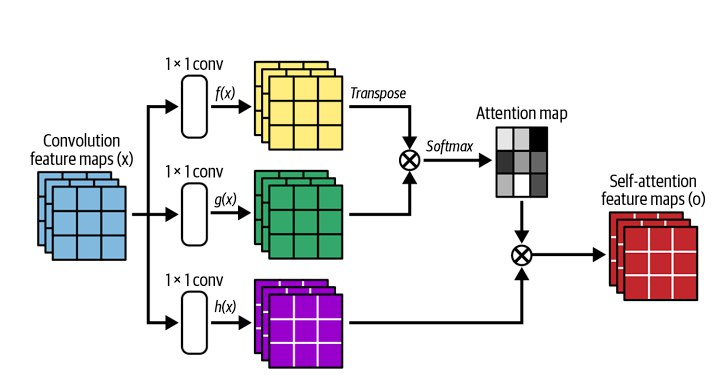
\includegraphics[scale=0.5]{task1/self-attn.jpg}}
            \\Self Attention Block
        \end{minipage}
        \begin{minipage}[t]{.5\textwidth}
            \centering
            \adjustbox{valign=t}{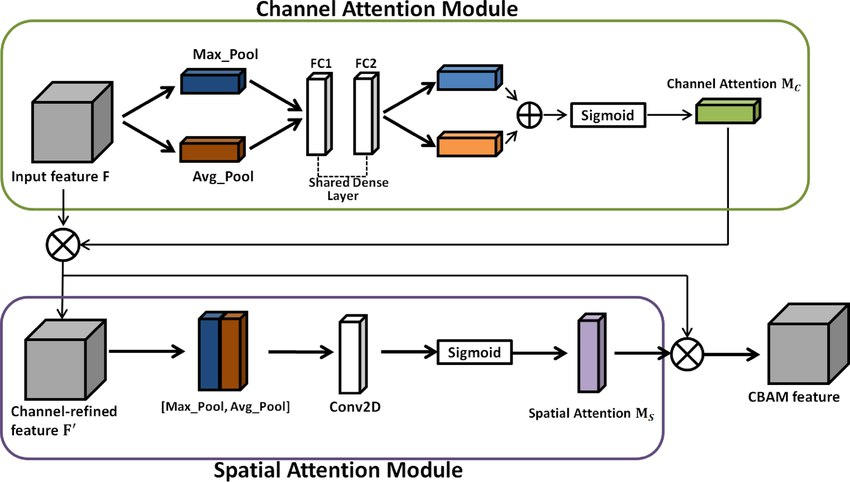
\includegraphics[scale=0.31]{task1/cbam.jpg}}
        \end{minipage}
    \end{fullwidth}
\end{figure}

% \newpage
\subsection{Discriminator}\label{task1:discriminator}
Our discriminator uses a basic sequential architecture with convolutional layers that doubles in number of channels 3 times, from 64 to 512. Each convolution output is passed to a spectral norm layer, instance normalisation and a leaky relu activation function. We then branched into a Avg Pool into a FC layer for global classification and a PatchGAN block for local classification. \\

\noindent Given that we have used a 256x256 image, the feature map will have size of $[B, 512, 16, 16]$, the patchGAN will have size of $[B, 1, 16, 16]$. A larger patch GAN and feature map allows us to capture more details of specific features in certain areas which allows the discriminator to provide more useful information to the generator.


\begin{figure}[h]
    \centering
    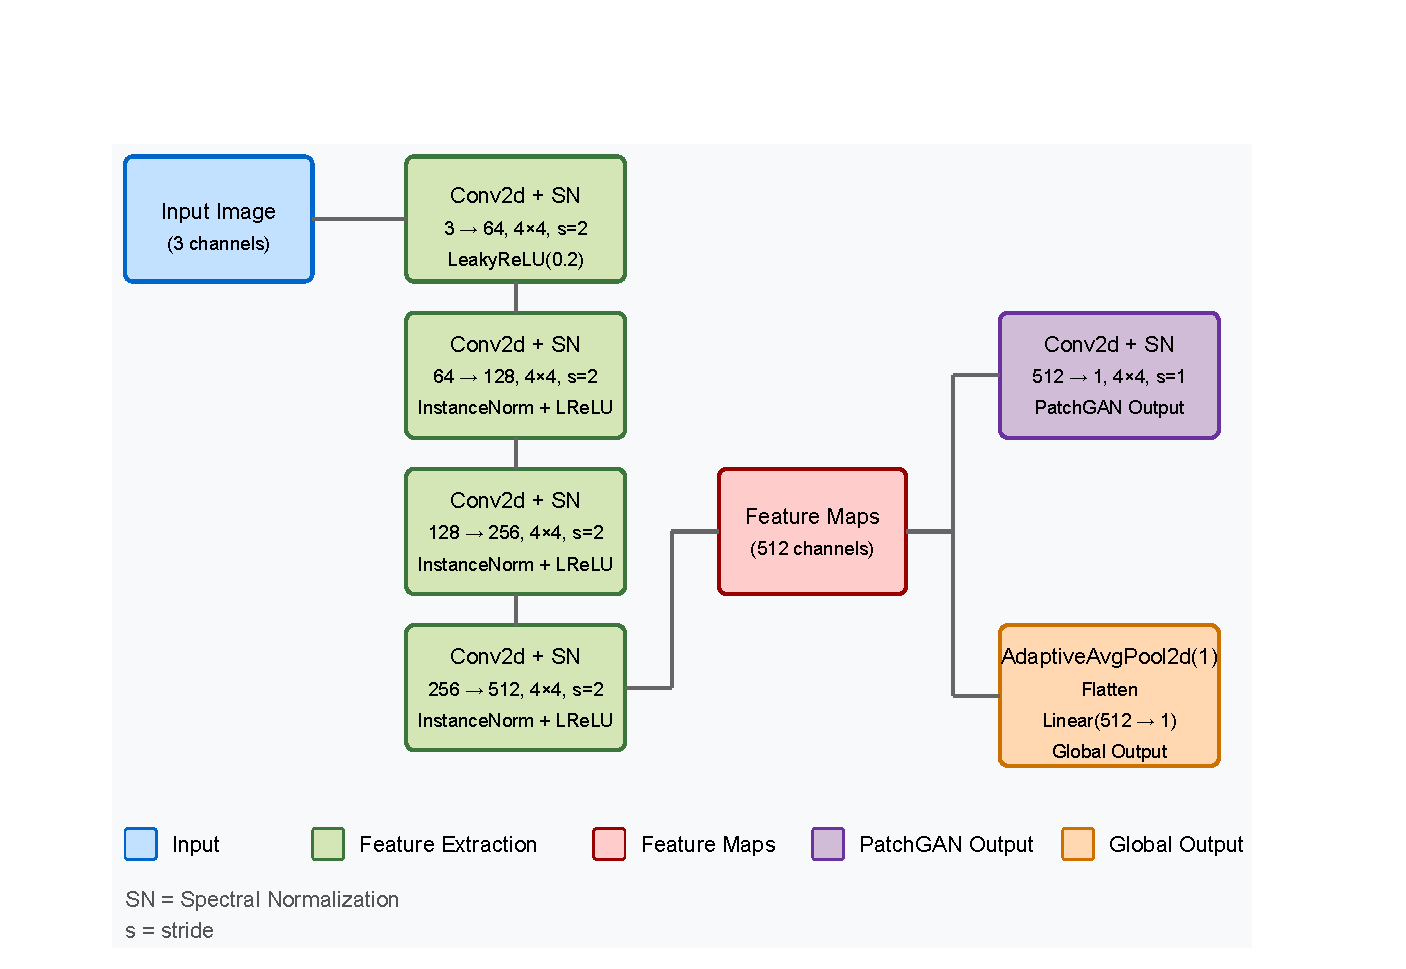
\includegraphics[width=0.7\textwidth]{task1/discriminator-architecture.pdf}
    \caption{Task 1: Discriminator Architecture}
\end{figure}


\section{Data Preparation}
\subsection{Augmentations}
We started with resizing images to 128x128, with a batch size of 16 before we hit a memory limit. We also applied no augmentations to the images, as a baseline to compare against later on when we add augmentations. \\

\noindent After adding various minor augmentations like affines, color jitters, flips, light gaussian blurs and posterising, we found that any combination of them resulted in worse metrics overall. From visual inspection, we found that the generated raw images were more noisy than without augmentations, which could contribute to the worse metrics. Furthermore, the generated cartoon images were a lot more flat than the target images, losing a lot more of the finer details and textures. Lastly, affines and any crops were clearly visible in the generated images when they otherwise should not be. \\

\noindent Thus, in both cases, we believe that adding the augmentations were encouraging the model to over-process the style conversions, which likely caused the reduction in metrics. Finally our best result was achieved with no augmentations, and upscaling the images to 256x256 with a batch size of 3. Some sample results are shown in the below Figures.

\begin{figure}[h]
    \centering
    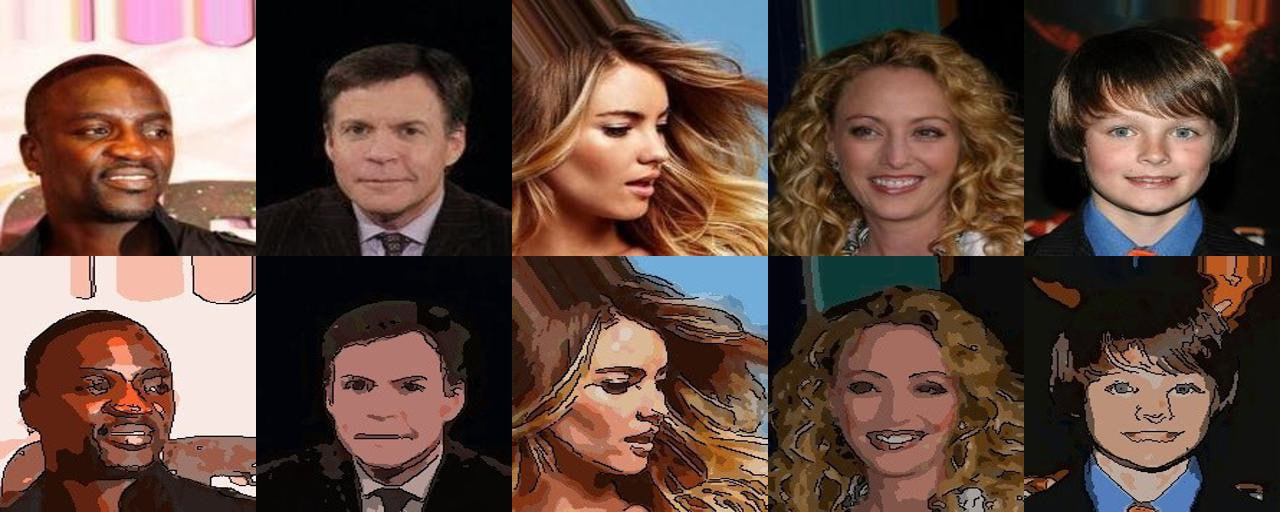
\includegraphics[width=0.8\linewidth]{task1/originals.jpg}
    \vspace{-10pt}
    \caption{Original (resized 256x256). Top row: Raw, Bottom row: Cartoon}
    \vspace{12pt}
    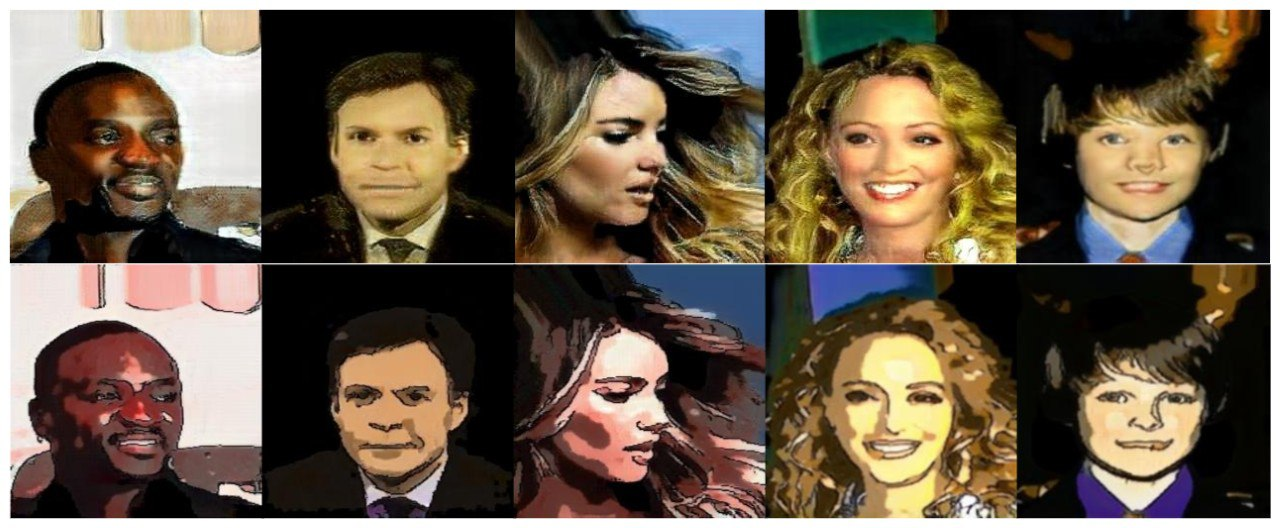
\includegraphics[width=0.8\linewidth]{task1/top2.jpg}
    \vspace{-10pt}
    \caption{128x128 Avg GMS: 4.47829}
    \vspace{12pt}
    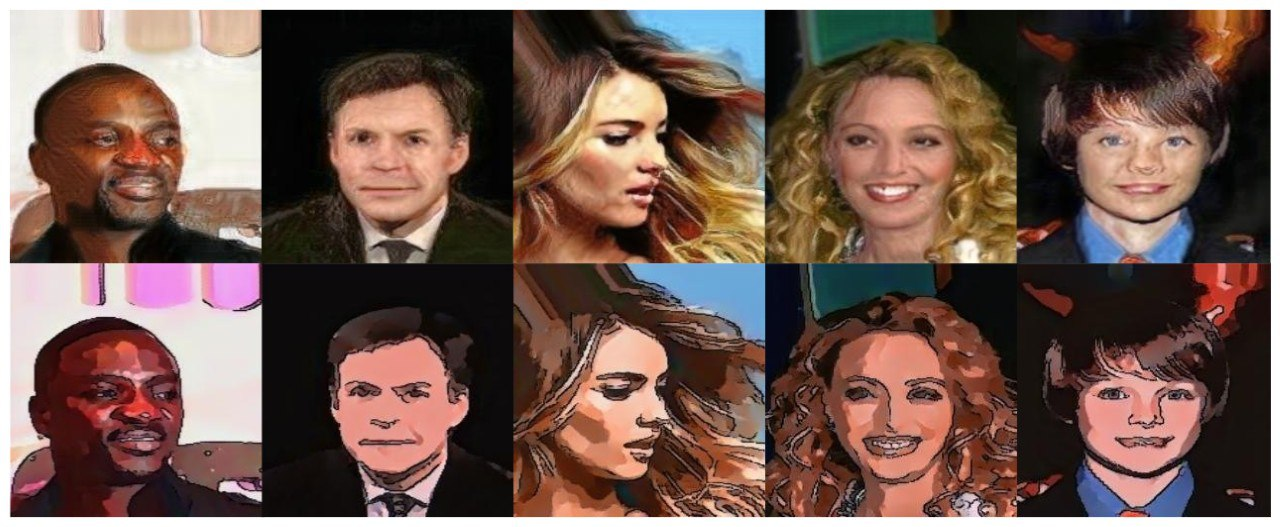
\includegraphics[width=0.8\linewidth]{task1/top1.jpg}
    \vspace{-10pt}
    \caption{256x256, Stage 1: Batch Size 3, Avg GMS: 3.72523}
    \vspace{12pt}
    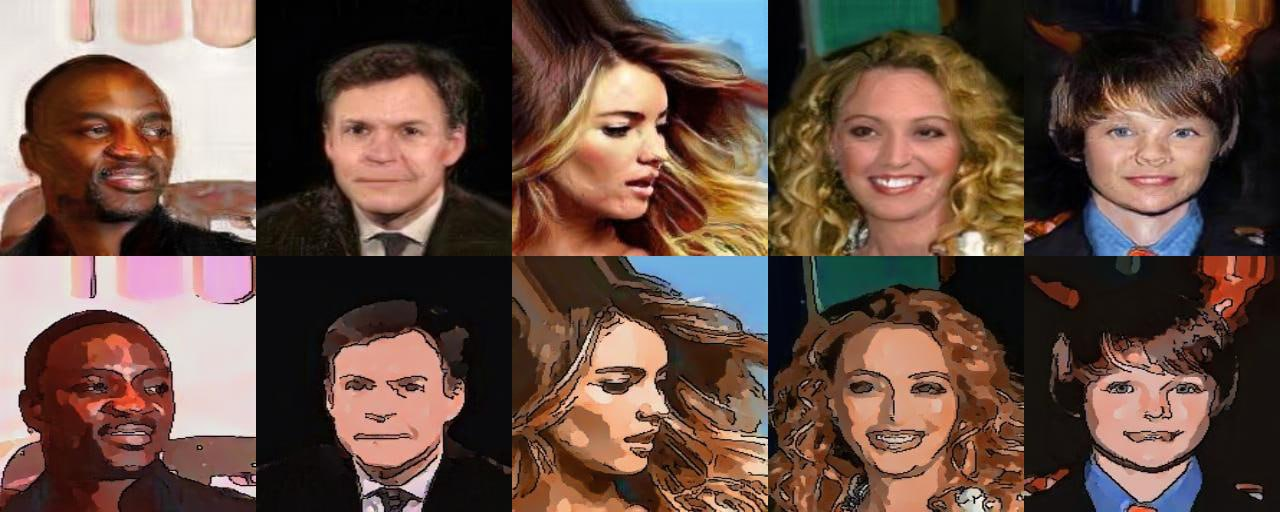
\includegraphics[width=0.8\linewidth]{task1/top3-3-42.jpg}
    \vspace{-10pt}
    \caption{256x256, Stage 2: Batch Size 2, Avg GMS: 3.42415}
\end{figure}

\subsection{Data Split}
We worked with simple 99/1 split on training/validation data since we found that we needed as much data as possible for training the model to achieve our best results. \\

\section{Methodology}

\subsection{Staged Training}\label{task1:staged-training}
Our best results came from a multi-staged supervised training approach. The idea is inspired from an application on Sketch-to-Manga colorization by Zhang et al. (2018)\footnote{Zhang, L., Li, C., Wong, T.-T., Ji, Y., \& Liu, C. (2018). Two-stage sketch colorization. ACM Transactions on Graphics, 261–261. \href{https://ttwong12.github.io/papers/colorize/colorize.pdf}{https://ttwong12.github.io/papers/colorize/colorize.pdf}}, where they utilised 2 generators using the same architecture, intended for them to have different focuses. 
Our methodology follows a "greedy" approach seen in \textbf{Algorithm \ref{alg:cap}} where we iteratively save checkpoints of our models, measure their metrics, and we keep the best performing weights. We then use these weights as a starting point for the next stage of training.
\paragraph*{\noindent Our novelty}stems from how we decrease the batch size, number of epochs, and evaluation threshold proportionally in each iterative stage, while using newly randomised seeds and maintaining learning rate so that our ratio of batch size to learning rate decreases\footnote{He, F., Liu, T., \& Tao, D. (2019). Control Batch Size and Learning Rate to Generalize Well: Theoretical and Empirical Evidence. In H. Wallach, H. Larochelle, A. Beygelzimer, F. d' Alché-Buc, E. Fox, \& R. Garnett (Eds.), Advances in Neural Information Processing Systems (Vol. 32). Retrieved from \\ \href{https://proceedings.neurips.cc/paper_files/paper/2019/file/dc6a70712a252123c40d2adba6a11d84-Paper.pdf}{https://proceedings.neurips.cc/paper\_files/paper/2019/file/dc6a70712a252123c40d2adba6a11d84-Paper.pdf}}. This allows us to gradually refine the model's performance and achieve better results as each iteration encourages the model to learn finer details. Our intention with newly randomised seeds was to allow the optimisers to start on a different location in the loss optimisation graph, which may force it to hit a new local minima. 

\begin{table}[h]
    \centering
    \begin{tabular}{|l|l|l|l|l|}
    \hline
    \textbf{Stage} & \textbf{Batch Sizes} & \textbf{Epochs} & \textbf{Eval Threshold} & \textbf{Torch Seed} \\
    \hline
    Stage 1 & 3 & 100 & 10 & 1722426635407800 \\
    Stage 2 & 2 & 50  & 10  & -- \\
    Stage 3 & 1 & 30  & 3  & -- \\
    \hline
    \end{tabular}
    \caption{Configuration of hyperparameters for each stage}
\end{table}

\begin{algorithm}[h]
    \caption{Basic Training Loop Single Stage}\label{alg:cap}
    \begin{algorithmic}
    \Procedure{trainModel}{$D^w_{A}, D^w_{B}, G^w_{AB}, G^w_{BA}, batchSize, epochs, evalThreshold$} \Comment{weights for models}
        \State $D_{A} \gets D^w_{A}$
        \State $D_{B} \gets D^w_{B}$
        \State $G_{AB} \gets G^w_{AB}$
        \State $G_{BA} \gets G^w_{BA}$
        \State $n \gets 1$
        \State $W\_history \gets [\quad]$
        \While{$n \neq epochs$}\Comment{Run basic training loop}
            \State$Train \quad D_{A}, D_{B}, G_{AB}, G_{BA} \quad with \quad Domain_A, Domain_B, batchSize$
            \If{$n \mod evalThreshold = 0$}
                \State $W\_history.insert({D^w_{A}, D^w_{B}, G^w_{AB}, G^w_{BA}})$
            \EndIf
            \State $n \gets n + 1$
        \EndWhile
        \State $bestGMS \gets inf$
        \State $bestW \gets {D^w_{A}, D^w_{B}, G^w_{AB}, G^w_{BA}}$
        \For{\texttt{$w_{e} \in W$}} \Comment{Evaluate each weight with test sets}
            \State $D_{A} \gets D^{w_{e}}_{A}$
            \State $D_{B} \gets D^{w_{e}}_{B}$
            \State $G_{AB} \gets G^{w_{e}}_{AB}$
            \State $G_{BA} \gets G^{w_{e}}_{BA}$
            \State $epochGMS \gets Compute \quad GMS$
            \If{$epochGMS < bestGMS$}
                \State $bestGMS \gets epochGMS$
                \State $bestW \gets w_{e}$
            \EndIf
        \EndFor
        \State \Return $bestW$ \Comment{Returns the best weights}
    \EndProcedure
    \end{algorithmic}
\end{algorithm}

\newpage
\subsection{Image Pooling}\label{task1:image-pooling}
An "Image Pool" was also used in training with a buffer of 50 images. This pool functions as a buffer to store previously generated images, which helps to reduce the risk of mode collapse where the Discriminator becomes too powerful, and prevents the Generator from learning anything new. The pool is updated with new generated fake images during training, and once the threshold is reached, we randomly sample from the available pool instead of using the latest generated image. 

\section{Loss Functions}\label{task1:losses}

\subsection{Discriminator Losses}
We used a combination of loss functions beyond the standard adversarial loss to improve the performance of our discriminator. Our overall loss function for the discriminator is as follows:
\begin{equation}
    L_{D} = L_{GAN} + \lambda_{gp} L_{gp}
\end{equation}

\subsubsection{Gradient Penalty – $L_{gp}$}
We also use a gradient penalty, inspired from Wasserstein GAN (WGAN)\footnote{Arjovsky, M., Chintala, S., \& Bottou, L. (2017, July 17). Wasserstein Generative Adversarial networks. PMLR. \href{https://proceedings.mlr.press/v70/arjovsky17a.html}{https://proceedings.mlr.press/v70/arjovsky17a.html}} in order to prevent the discriminator from learning too fast. Doing so avoids problems like mode collapse with vanishing gradients, and ensures that the generator is always learning, even if it is not performing well enough to "beat" the discriminator yet, thus improving stability of training.
\begin{equation*}
    \text{Gradient Penalty Loss} = 0.7 \cdot \mathbb{E} \left[ \left( \| \nabla_{\hat{x}} D_{\text{patch}} (\hat{x}) \|_2 - 1 \right)^2 \right] + 0.3 \cdot \mathbb{E} \left[ \left( \| \nabla_{\hat{x}} D_{\text{global}} (\hat{x}) \|_2 - 1 \right)^2 \right]
\end{equation*}

\subsubsection{Relativistic – $L_{GAN}$}
We extend the typical adversarial loss by using a relativistic loss, which compares the logits of discriminating the real and fake images in a relative manner on a global scope with Binary Cross Entropy Loss. Furthermore, we took inspiration from PatchGAN\footnote{Isola, P., Zhu, J., Zhou, T., \& Efros, A. A. (2016). Image-to-Image Translation with Conditional Adversarial Networks. arXiv (Cornell University). \href{https://doi.org/10.48550/arxiv.1611.07004}{https://doi.org/10.48550/arxiv.1611.07004}} which whether the images is real or fake based on smaller patches, a local scope. Thus, we have another source of information for determining real or fake, which is computed with MSE loss. The equation for our relativistic loss for our "real" side is as follows, and the opposite will be applied for the "fake" side i.e. $D_{real} <=> D_{fake}, True <=> False$:
\begin{equation}
    L_{GAN} = 0.7 \cdot MSE(D_{real} - \bar{D}_{fake}, True)_{patch} + 0.3 \cdot BCE(D_{real} - \bar{D}_{fake}, True)_{global}
\end{equation}

\subsection{Generator Losses}
The generator also makes use of the \textbf{Relativistic} loss, which is an extension of the standard adversarial GAN loss. Our overall loss function for the generator is as follows:
\begin{equation}
    L_{G} = L_{GAN} + \lambda_{cyc} L_{cyc} + \lambda_{id} L_{id} + \lambda_{feat} L_{feat}
\end{equation}
\subsubsection{Cycle Consistency – $L_{cyc}$}
As we would like the fake images to be able revertible to its original image i.e. the pixels are identical, we maintain using L1 Loss for our Cycle Consistency.

\subsubsection{Identity – $L_{id}$}
Similarly, we also use L1 Loss for our Identity loss since images in the same domain should not be altered. 
\subsubsection{Feature – $L_{feat}$}
Another extension that we incorporated is the Feature Loss, which serves as a perceptual loss that compares the features of the generated image with the target image. Although traditionally used with pre-trained networks, we used the features extracted from the training discriminator instead. These features are compared using L1 loss, which helps to ensure that the generated images are perceptually similar to the target images. 

\section{Conclusion}
In summary, our work extends the typical CycleGAN framework with significant enhancements to both architecture and training methodology. By integrating advanced attention mechanisms and refined normalization techniques (see \ref{task1:generator}), and adopting a multi-staged training approach with strategically adjusted hyperparameters (see \ref{task1:staged-training}), we achieved significantly improved image quality, from METRIC1 down to METRIC2. The combined use of gradient, adversarial, cycle consistency, identity, and feature losses (see \ref{task1:losses}) further stabilised training and perceptual realism. 

\section{Appendix}\label{task1:appendix}

\begin{figure}[h]
    \centering
    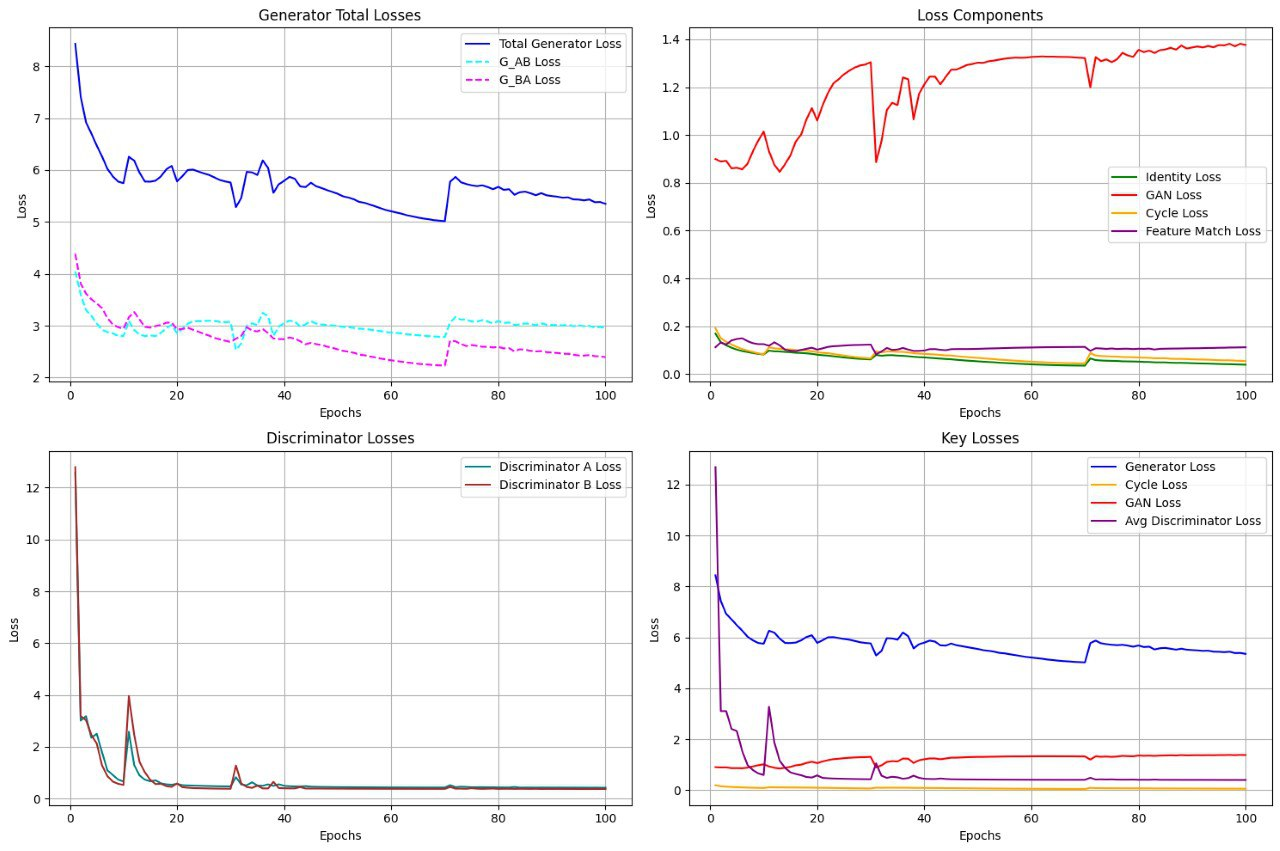
\includegraphics[width=\textwidth]{task1/stage1_loss.jpg}
    \vspace{-10pt}
    \caption{Loss curve for Stage 1 training}
    \vspace{12pt}
    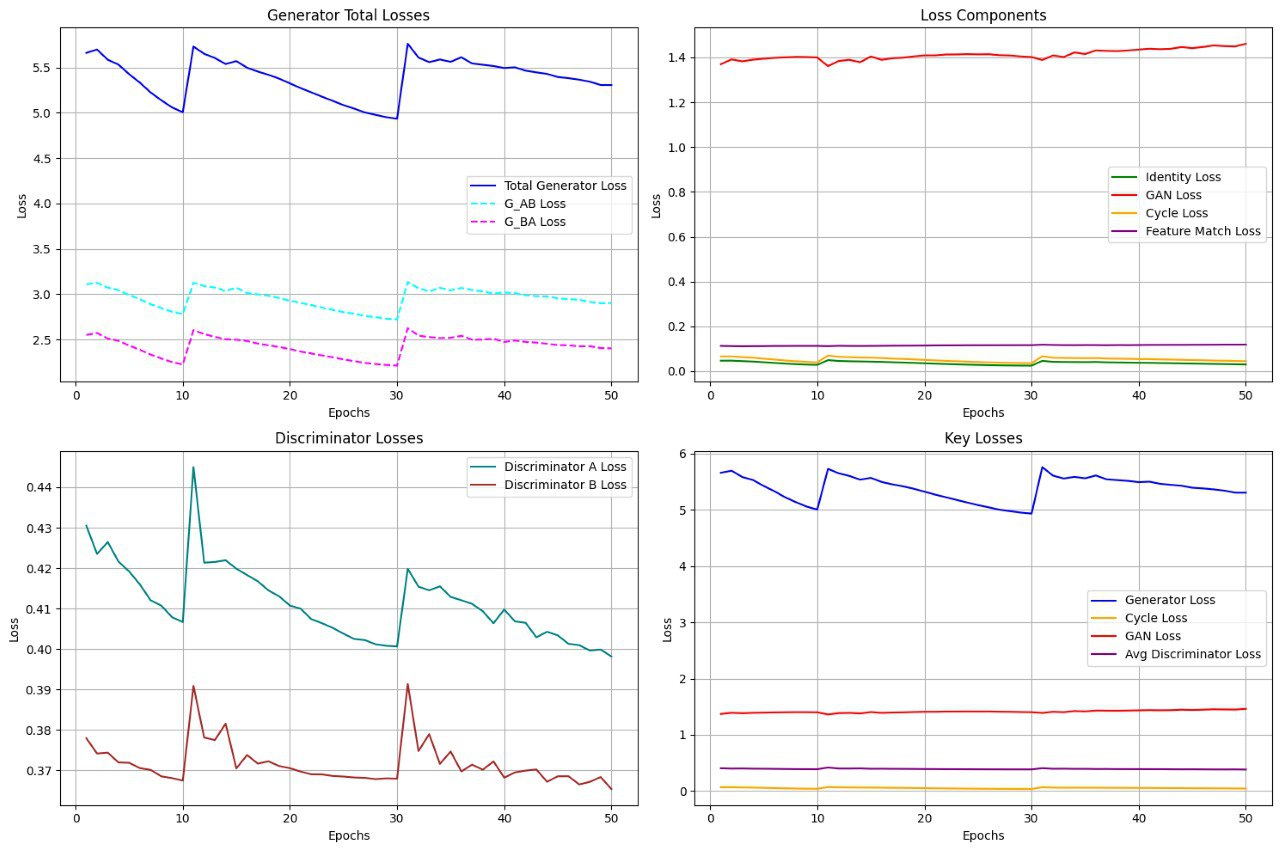
\includegraphics[width=\linewidth]{task1/stage2_loss.jpg}
    \vspace{-10pt}
    \caption{Loss curve for Stage 2 training}
    \vspace{12pt}
\end{figure}

\begin{table}[h]
    \centering
    \begin{tabular}{|l|c|c|c|c|}
    \hline
    \textbf{Stage / Direction} & \textbf{FID} $\downarrow$ & \textbf{IS} $\uparrow$ & \textbf{GMS} $\downarrow$ & \textbf{Avg GMS} $\downarrow$ \\
    \hline
    \multicolumn{5}{|c|}{\textbf{Stage 1}} \\
    \hline
    Raw to Cartoon     & 46.70193     & 2.41466 ± 0.24392   & 4.39783    & \multirow{2}{*}{3.85666} \\
    Cartoon to Raw     & 39.83461         & 3.62382 ± 0.23992        & 3.31548        &            \\
    \hline
    \multicolumn{5}{|c|}{\textbf{Stage 2}} \\
    \hline
    Raw to Cartoon     & 31.6551     & 2.2699 ± 0.20   & 3.7344    & \multirow{2}{*}{3.42423} \\
    Cartoon to Raw     & 35.1988     & 3.6300 ± 0.22   & 3.1139    &            \\
    \hline
    \multicolumn{5}{|c|}{\textbf{Stage 3}} \\
    \hline
    Raw to Cartoon     & TBC     & TBC ± 0.18   & TBC    & \multirow{2}{*}{TBC} \\
    Cartoon to Raw     & TBC     & TBC ± 0.21   & TBC    &            \\
    \hline
    \end{tabular}
    \caption{Evaluation metrics across stages, best results taken from each stage}
    \label{tab:staged-eval}
\end{table}



\chapter{Task 2}
\section{Introduction}



\subsection{Configuration}\label{task2:configuration}

All optimisers used Adam with a Cosine Annealing Warm Restarts scheduler. The following hyperparameters and loss weights were used for our best results:

\begin{multicols}{3}
    \begin{itemize}
        \item Random seed: 42
        \item Epochs: 501
        \item Batch size: 32
        \item Learning rate: 3e-4
        \item Betas: (0.5, 0.999)
        \item $Scheduler_{t-0}$: 10
        \item $Scheduler_{t-mult}$: 2
        \item $Scheduler_{min-lr}$: 1e-5
        \item $\lambda_{cyc}$: 6.0
        \item $\lambda_{id}$: 3.0
        \item $\lambda_{gan}$: 1.0
        \item $\lambda_{gp}$: 10.0
        \item $\lambda_{fm}$: 8.0
        \item $\lambda_{perceptual}$: 2.0
    \end{itemize}
\end{multicols}



\section{Architecture}
\subsection{Generator}\label{task2:generator}
We used a similar architecture as the one used in Task 1 (\ref{task1:generator}) for our best results. The following parameters were also used for our generator:

\begin{multicols}{3}
    \begin{itemize}
        \item Residual Blocks: 6
        \item Use Attention: True
        \item Features Dimension: 64
    \end{itemize}
\end{multicols}

\paragraph{Failure From VQGAN Implementation:} 

\textbf{Vector Quantization Block}\ref{fig:vq-concept} is used to convert the input image into a discrete representation, which is then passed through a series of residual blocks. The output of the residual blocks is then passed through a decoder to reconstruct the image. The vector quantization block is used to learn a set of discrete codes that can be used to represent the input image, allowing for more efficient encoding and decoding. 

which will learn additional features, as animal and pokemon do not have a direct translation.



\subsection{Discriminator}\label{task2:discriminator}
We used the same general architecture as the one used in Task 1 (\ref{task1:discriminator}), with a few modifications specific to catering for the smaller images. Since our Pokémon sprite sizes are only 96x96, we removed the last downsampling layer of the discriminator so bottleneck/features will be capped at $[B, 256, 12, 12]$.
\noindent The reasons are two-fold: 

\begin{itemize}
    \item The structure of an animal and pokemon being very different, so we will not want to make the discriminator too powerful. 
    \item A $[B, 256, 6, 6]$ feature map will not provide enough useful information to the generator either, thus a $[B, 256, 12, 12]$ feature map can better help the generator to identify the Pokémon sprite style.
\end{itemize}


\begin{figure}[h]
    \centering
    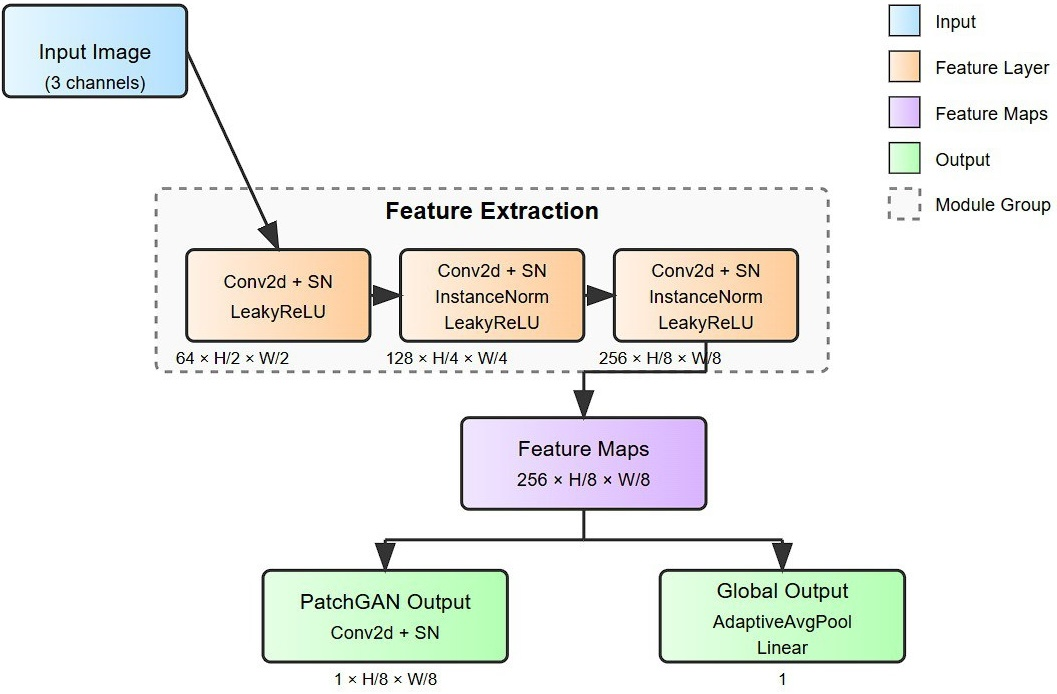
\includegraphics[width=0.7\textwidth]{task2/discriminatorArchitecture.jpg}
    \caption{Task 2: Discriminator Architecture}
\end{figure}



\section{Data Preparation}
\subsection{Collection}
Due to our task of transfering the styles from a real-life animal to that of a Pokémon sprite, we were unable to find a paired dataset between these 2 domains. Thus, we resorted to utilising 2 individual datasets: one for the animal images, another for the Pokémon sprites, and then combining them together.

\subsubsection{Animal Dataset}
The animal dataset \footnote{Animal Image Dataset (90 Different Animals) – Zooming in on Wildlife: 5400 Animal Images Across 90 Diverse Classes \href{https://www.kaggle.com/datasets/iamsouravbanerjee/animal-image-dataset-90-different-animals}{https://www.kaggle.com/datasets/iamsouravbanerjee/animal-image-dataset-90-different-animals}} we used consists of 5400 images of animals from 90 different classes / types of animals. We decided to use all images from the animal dataset. (Usability: 10.0 Total Image: 5.4k)



\subsubsection{Pokémon Sprite Dataset}
We decided to use Pokémon sprites as comapared to the original Pokémon art as we there is a distinct style to how Pokémon sprites are. Furthermore, using the original Pokémon art would not be suitable for a "style transfer" as we felt that the original art is at the prerogative of the individual artists when they created them. Thus, the styles across Pokémon will not be consistent, and our model will find it very difficult to learn the mapping between the two domains. Our failed attempts can be seen in Figure \ref{fig:poke-fail1} using this dataset\footnote{All Pokemon Official Artworks – A Comprehensive Dataset of All 1010 Official Pokémon Artworks \href{https://www.kaggle.com/datasets/hesselaar/all-pokemon-official-images}{https://www.kaggle.com/datasets/hesselaar/all-pokemon-official-images}}

\begin{figure}[h]
    \centering
    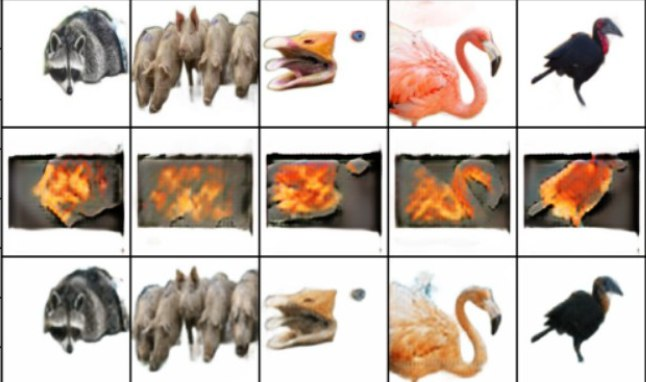
\includegraphics[width=0.7\textwidth]{task2/poke-fail1.jpg}
    \vspace{-10pt}
    \caption{Unacceptable style transfer with Pokémon Official Art}\label{fig:poke-fail1}
\end{figure}

\noindent Notice that the generated image does not resemble Pokémon art at all. We suspect that it is trying to colour the animal images in but it does not know exactly in what colour to use, and it does not make any informed or uninformed strong decision on how to colour. Thus, it ended up looking like a "mash-up" of the two domains, using the exact same colouring pattern. 

\noindent Thus, we finalised on using the Pokémon sprite dataset \footnote{Pokemon sprite images – Total 10,437 Pokemon sprite images in 96x96 resolution. \\ \href{https://www.kaggle.com/datasets/yehongjiang/pokemon-sprites-images}{https://www.kaggle.com/datasets/yehongjiang/pokemon-sprites-images}} that consists of many different variations of the same Pokémon, namely those front-facing, back facing, shiny and normal. We have decided to use the normal and front-facing versions as those are the most suitable given that our animal datasets also exhibit the same characteristics. (Usability 5.29, Total Image: 10.2k)

\subsection{Pre-Processing}\label{task2:preprocess}
Due to the domains being vastly different, and the images are of different formats, we had to pre-process the images before feeding them into the model so that it will learn what it needs to learn. 
\subsubsection{Background Removal}
The Pokémon sprites from the dataset are placed on a white background, whereas the animal images are not. Thus, we need to remove the background of the animal images so that the model can focus on the animals themselves rather than including how to convert the background to white. \\

\noindent To do so, we used a pretrained model (VGG16) to remove the background of the animal and convert them into white background found in \verb|clean_background.py|.

\subsubsection{No Tightly Paired Images}
We \textbf{randomly} paired each animal to a \textbf{random} Pokémon and we ensure that each Pokémon is not used too many times, as the different Pokémons are not equally represented in quantity. Since we have 1025 unique Pokémon, with different quantity of front-facing Pokémons, and 5400 different animal images, we try to ensure that each type of Pokémon sprite is at most represented 6 times. Finally, we have a total of 5400 animal-Pokémon paired images. 

\paragraph{Failure From Tight Pairs:} Before choosing to adopt a more "unsupervised learning" approach, we tried to mimic a "supervised learning" by mapping the animals to a specific Pokémon based on how similar their general designs are. However, we found that the results were \textbf{not satisfactory}. Although it does look like a Pokémon sprite from afar, it has a much worse GMS score as compared to the non-tightly paired dataset. Furthermore, we also conducted an anonymised field test through telegram polling with students across various schools-NUS, SMU, NTU-where some specifically are involved in Pokémon clubs, and across various undergraduate years. As of writing, we have 131 responses, with $1.5x$ more people prefer the results from the randomly-paired dataset compared to the tightly paired dataset. The methodology of the poll can be found in Appendix \ref{fig:survey}. Thus, it was sufficiently convincing for us to use the randomly paired dataset method.

\begin{figure}[h]
    \centering
    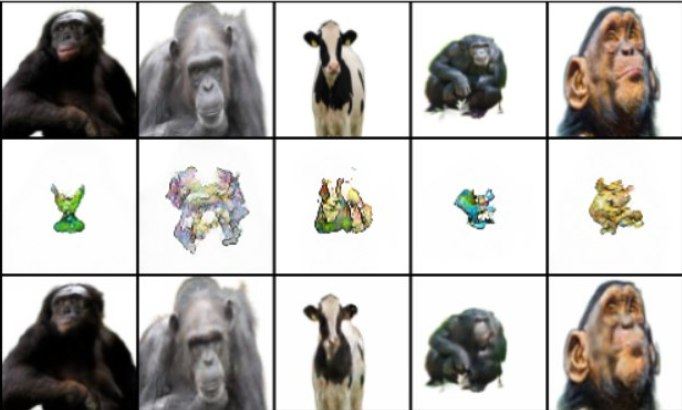
\includegraphics[width=\textwidth]{task2/poke-fail2.jpg}
    \vspace{-10pt}
    \caption{Unsatisfactory results from tightly paired dataset}
\end{figure}


\subsection{Data Split}

We split the pre-processed dataset into a simple 90/10 train-test split. So, we will have 4860 train images and 540 test images. The training set (4860 images) is split further to a 99/1 split, where 4811 images will be used for training, while 49 will be used for validation (visualisation of how the pokemon will look like). 


\section{Loss Functions}
Our loss functions for task 2 is identical to that of task 1 \textbf{with the exception of an additional loss, Perceptual Loss \ref{task2:generator:loss:perceptual}, for our Generator } In summary, we used a combination of loss functions beyond the standard set of losses in a CycleGAN. 

\subsection{Discriminator Losses}
We used a combination of loss functions beyond the standard adversarial loss to improve the performance of our discriminator. Our overall loss function for the discriminator is as follows:
\begin{equation}
    L_{D} = L_{GAN} + \lambda_{gp} L_{gp}
\end{equation}

\subsubsection{Gradient Penalty – $L_{gp}$}
We also use a gradient penalty, inspired from Wasserstein GAN (WGAN)\footnote{Arjovsky, M., Chintala, S., \& Bottou, L. (2017, July 17). Wasserstein Generative Adversarial networks. PMLR. \href{https://proceedings.mlr.press/v70/arjovsky17a.html}{https://proceedings.mlr.press/v70/arjovsky17a.html}} in order to prevent the discriminator from learning too fast. Doing so avoids problems like mode collapse with vanishing gradients, and ensures that the generator is always learning, even if it is not performing well enough to "beat" the discriminator yet, thus improving stability of training.
\begin{equation*}
    \text{Gradient Penalty Loss} = 0.7 \cdot \mathbb{E} \left[ \left( \| \nabla_{\hat{x}} D_{\text{patch}} (\hat{x}) \|_2 - 1 \right)^2 \right] + 0.3 \cdot \mathbb{E} \left[ \left( \| \nabla_{\hat{x}} D_{\text{global}} (\hat{x}) \|_2 - 1 \right)^2 \right]
\end{equation*}

\subsubsection{Relativistic – $L_{GAN}$}
We extend the typical adversarial loss by using a relativistic loss, which compares the logits of discriminating the real and fake images in a relative manner on a global scope with Binary Cross Entropy Loss. Furthermore, we took inspiration from PatchGAN\footnote{Isola, P., Zhu, J., Zhou, T., \& Efros, A. A. (2016). Image-to-Image Translation with Conditional Adversarial Networks. arXiv (Cornell University). \href{https://doi.org/10.48550/arxiv.1611.07004}{https://doi.org/10.48550/arxiv.1611.07004}} which whether the images is real or fake based on smaller patches, a local scope. Thus, we have another source of information for determining real or fake, which is computed with MSE loss. The equation for our relativistic loss for our "real" side is as follows, and the opposite will be applied for the "fake" side i.e. $D_{real} <=> D_{fake}, True <=> False$:
\begin{equation}
    L_{GAN} = 0.7 \cdot MSE(D_{real} - \bar{D}_{fake}, True)_{patch} + 0.3 \cdot BCE(D_{real} - \bar{D}_{fake}, True)_{global}
\end{equation}

\subsection{Generator Losses}
The generator also makes use of the \textbf{Relativistic} loss, which is an extension of the standard adversarial GAN loss. It also takes advantage of a pre-trained VGG16 model to compare the similarities of extracted, as referenced earlier as \textbf{Perceptual Loss}. Our overall loss function for the generator is as follows:
\begin{equation}
    L_{G} = L_{GAN} + \lambda_{perceptual} L_{perceptual} + \lambda_{cyc} L_{cyc} + \lambda_{id} L_{id} + \lambda_{feat} L_{feat}
\end{equation}

\subsubsection{Perceptual Loss – $L_{perceptual}$}\label{task2:generator:loss:perceptual}
We used a perceptual loss, which is a combination of the content and style loss. The content loss is computed using the features extracted from the VGG16 model, while the style loss is computed using the Gram matrix of the features. The perceptual loss helps to ensure that the generated images are perceptually similar to the target images, while also maintaining the overall structure and content of the images.

\subsubsection{Cycle Consistency – $L_{cyc}$}
As we would like the fake images to be able revertible to its original image i.e. the pixels are identical, we maintain using L1 Loss for our Cycle Consistency.

\subsubsection{Identity – $L_{id}$}
Similarly, we also use L1 Loss for our Identity loss since images in the same domain should not be altered. 
\subsubsection{Feature – $L_{feat}$}
Another extension that we incorporated is the Feature Loss, which serves as a perceptual loss that compares the features of the generated image with the target image. Although traditionally used with pre-trained networks, we used the features extracted from the training discriminator instead. These features are compared using L1 loss, which helps to ensure that the generated images are perceptually similar to the target images. 

\section{Methodology}
Similar to task 1, we also made use of \textbf{Image Pooling} (as seen in \ref{task1:image-pooling}). However, we did not employ any additional special training techniques due to the lack of time to experiment. Instead, we opted for the standard training procedure with the hyperparameters as mentioned in \ref{task2:configuration}.
% \subsection{Image Pooling}
% An "Image Pool" was also used in training. This pool functions as a buffer to store previously generated images, which helps to reduce the risk of mode collapse where the Discriminator becomes too powerful, and prevents the Generator from learning anything new. The pool is updated with new generated fake images during training, and once the threshold is reached, we randomly sample from the available pool instead of using the latest generated image. 

\section{Metrics}\label{task2:metrics}

\begin{table}[h]
    \centering
    \caption{Evaluation Metrics for Animal $\rightarrow$ Pokémon Style Transfer}
    \begin{tabular}{lcccccc}
        \hline
        \textbf{Model} & 
        \textbf{FID} $\downarrow$ & 
        \textbf{IS} $\uparrow$ & 
        \textbf{GMS} $\downarrow$ & 
        \textbf{SSIM} $\uparrow$ & 
        \textbf{Perceptual} $\downarrow$ & 
        \textbf{Diversity} $\uparrow$ \\
        \hline
        Animal $\rightarrow$ Pokémon    & 96.37582 & 2.50949 ± 0.24199 & 6.19713 & 0.7262 & 3.0451 & 0.1451 \\
        Pokémon $\rightarrow$ Animal       & 205.14336 & 3.26938 ± 0.30883 & 7.92128 & 0.5977 & 2.7445 & 0.2408 \\
        \hline
    \end{tabular}
    \label{tab:metrics}
\end{table}

\section{Conclusion}
In summary, our work inherits the learnings from Task 1 by introducing modifications tailored to the more challenging domain translation between animal images and Pokémon sprites. Key enhancements include the incorporation of a Vector Quantization Block for efficient encoding (see \ref{task2:generator}) and adjustments to the discriminator architecture to accommodate smaller image resolutions (see \ref{task2:discriminator}). Our data preparation strategy—featuring background removal and randomized pairing (see \ref{task2:preprocess})—ensured the model could efficiently learn the differences between the two domains. Finally, by integrating an additional Perceptual Loss into our loss functions (see \ref{task2:generator:loss:perceptual}), we further improved the perceptual fidelity of the generated images while maintaining training stability as seen from our metrics, utilising both subjective and objective analysis (see \ref{task2:metrics}). These innovations together present a robust solution for unsupervised style transfer between highly disparate visual domains.


\section{Appendix}

\subsection{Randomly Paired vs Supervised Paired Dataset Preference}

\begin{figure}[h]
    \centering
    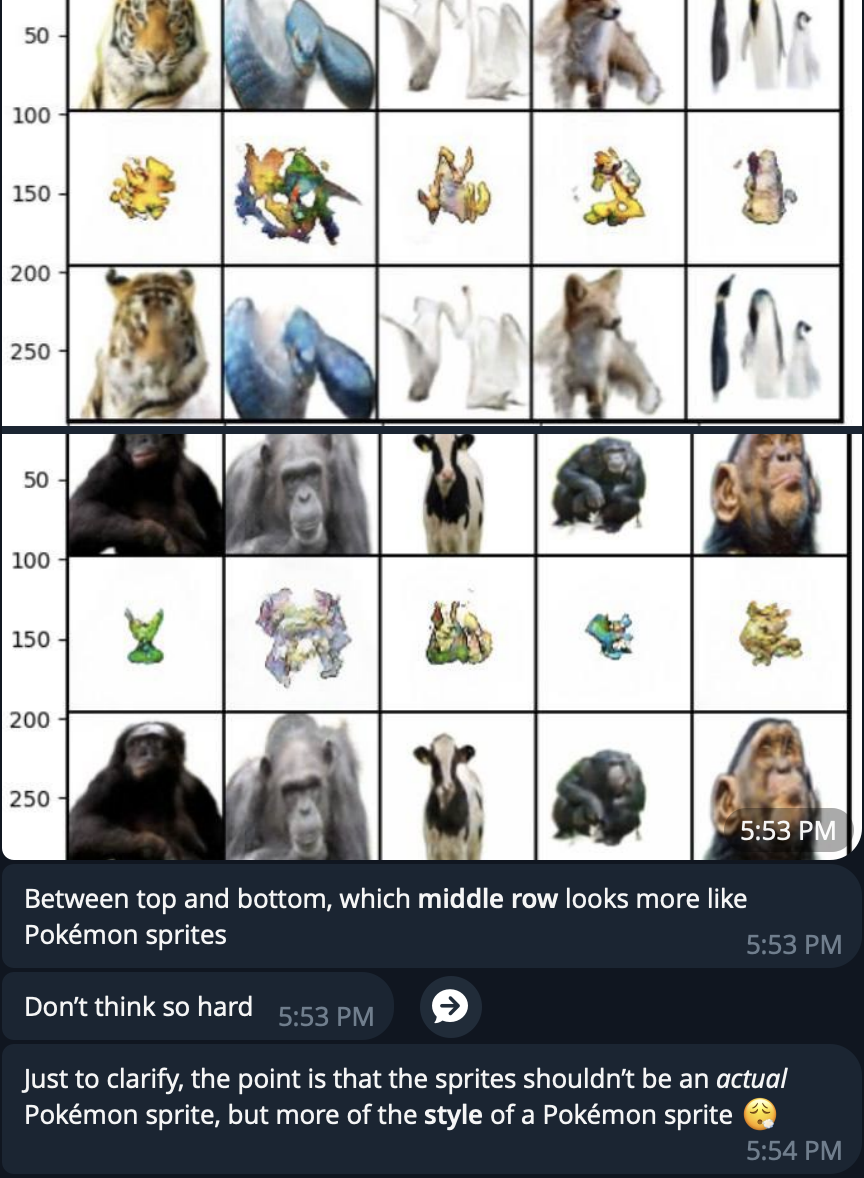
\includegraphics[width=0.7\textwidth]{task2/subjectivePolling.png}
    \vspace{-10pt}
    \caption{Context given to polling participants}
    \vspace{12pt}
    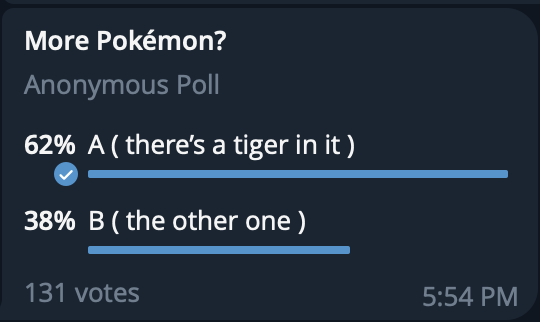
\includegraphics[width=0.7\textwidth]{task2/surveyResults.png}
    \vspace{-10pt}
    \caption{Poll Results}
    \vspace{12pt}
    \label{fig:survey}
\end{figure}

\begin{figure}[h]
    \centering
    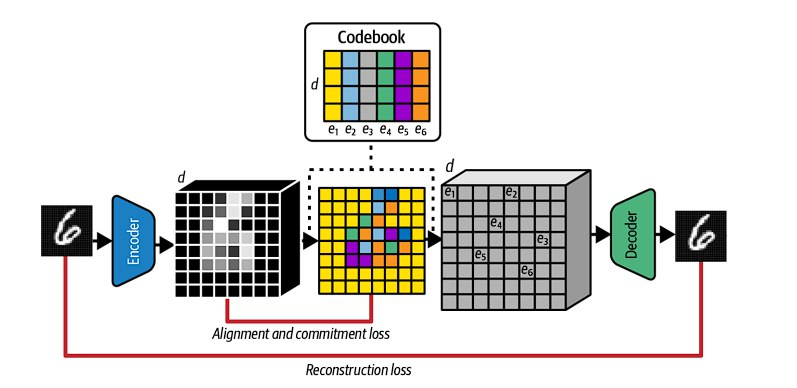
\includegraphics[width=\textwidth]{task2/vq-block.jpg}
    \caption{Vector Quantization Block}
    \label{fig:vq-concept}
\end{figure}


\begin{figure}[h]
    \centering
    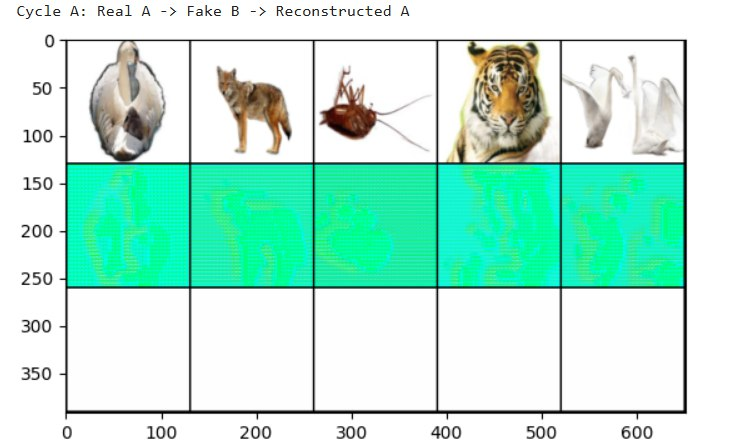
\includegraphics[width=0.7\textwidth]{task2/failedvq1.jpg}
    \vspace{-10pt}
    \caption{Complete failure of VQGAN for Animals $\rightarrow$ Pokémon $\rightarrow$ Reconstructed Animals}
    \vspace{12pt}
    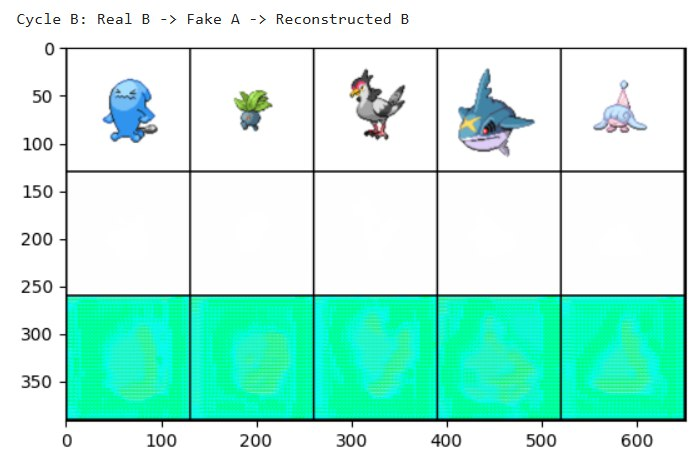
\includegraphics[width=0.7\textwidth]{task2/failedvq2.jpg}
    \vspace{-10pt}
    \caption{Complete failure of VQGAN for Pokémon $\rightarrow$ Animals $\rightarrow$ Reconstructed Pokémon}
    \vspace{12pt}
    \label{fig:failed-vq}
\end{figure}


\bibliographystyle{plain}
\bibliography{references}  % Create a references.bib file with your citations

\end{document}